\newpage
\chapter{Pregled korištenih programskih jezika i idioma} \label{chpt:first}

U ovom su poglavlju detaljno opisani programski jezici, tehnike i komunikacijski
protokoli koji su korištene pri izradi diplomskoga rada.

\begin{figure}[H]
\centering
\begin{tikzpicture}
    \node[draw=OliveGreen, rectangle, minimum width=120, minimum height=200,
    label={[label distance=-180, font=\Large\bf, color=white]-90:Plant},
    fill=OliveGreen, rounded corners]
    (plant) {};

    \node[draw=MidnightBlue, rectangle, minimum width=120, minimum height=200,
    label={[label distance=-180, font=\Large\bf, color=white]-90:Server},
    fill=MidnightBlue, rounded corners, right=1.5 of plant]
    (daemon) {};

    \node[draw=DarkOrchid, rectangle, minimum width=120, minimum height=200,
    label={[label distance=-180, font=\Large\bf, color=white]-90:Client},
    fill=DarkOrchid, rounded corners, right=1.5 of daemon]
    (client) {};

    \node[draw=LimeGreen, rectangle, rounded corners, minimum height=40,
          minimum width=100, fill=LimeGreen, below=-5 of plant, font=\bf]
          (arduino) {\textcolor{white}{Microcontroller}};

    \node[draw=LimeGreen, rectangle, rounded corners, minimum height=40,
          minimum width=100, fill=LimeGreen, below=1.5 of arduino, font=\bf]
          (process) {\textcolor{white}{Process}};

    \node[draw=NavyBlue, rectangle, rounded corners, minimum height=40,
          minimum width=100, fill=NavyBlue, below=-5 of daemon, font=\bf]
          (regulator) {\textcolor{white}{Regulator}};

    \node[draw=NavyBlue, rectangle, rounded corners, minimum height=40,
          minimum width=100, fill=NavyBlue, below=1.5 of regulator, font=\bf]
          (sserver) {\textcolor{white}{Socket Server}};

    \node[draw=Thistle, rectangle, rounded corners, minimum height=40,
          minimum width=100, fill=Thistle, below=-5 of client, font=\bf]
          (UI) {\textcolor{white}{UI}};

    \node[draw=Thistle, rectangle, rounded corners, minimum height=40,
          minimum width=100, fill=Thistle, below=1.5 of UI, font=\bf]
          (sclient) {\textcolor{white}{Socket Client}};

    \draw[Latex-Latex, line width=2, color=Peach] (arduino) to (regulator);
    \draw[Latex-Latex, line width=2, color=Peach] (arduino) to (process);
    \draw[Latex-Latex, line width=2, color=Peach] (arduino) to (process);
    \draw[Latex-Latex, line width=2, color=Peach] (sserver) to (sclient);
    \draw[Latex-Latex, line width=2, color=Peach] (regulator) to (sserver);
    \draw[Latex-Latex, line width=2, color=Peach] (UI) to (sclient);
\end{tikzpicture}
\caption{Shematski prikaz rada}
\label{fig:main_sheme}
\end{figure}

Na slici \ref{fig:main_sheme} je prikazan sinopsis diplomskoga rada koji je podijeljen u 3 dijela:
\begin{itemize}
        \item Postrojenje
        \item Server
        \item Klijent
\end{itemize}

Kao što je već spomenuto u poglavlju \ref{introduction}, postrojenje se sastoji
od mikroupravljača i dviju boca koje služe kao model za održavanje razine vode.

Server, koji je pisan u Haskellu, također se sastoji od dva dijela, regulatora i
socket servera. Regulacijski dio s postrojenjem komunicira pomoću Firmata
protokola, a socket server s klijentima komunicira pomoću JSON-RPC protokola.

Klijent koji je pisan u Pythonu sastoji se od korisničkog sučelja i socket
klijenta koji periodički dohvaća trenutno stanje postrojenja od servera.

\section{Haskell}

Haskell je moderan, standardan, nije striktan, čisto funkcionalan programski
jezik. Dizajniran je za širok spektar primjena, od numeričkih do
simboličkih \cite{haskell_intro}.

Haskell je nastao 1990. godine te nakon nekoliko godina razvoja glavne osobine
bile su mu \cite{haskell_history}:

\begin{itemize}
\item Statički pisan
\item Sigurnost tipova
\item Lijenost
\item Klase tipova.
\end{itemize}

Statički pisan jezik zahtijeva da pri kompilaciji koda svi tipovi podataka budu
poznati, što donosi niz prednosti kao primjećivanje grešaka prije nego što se
program izvrši, efikasniji kod jer compiler zna unaprijed veličinu podataka,
nije potrebno provjeravati tip podatka dok se program izvršava.

Sigurnost tipova proizlazi iz strogo statičkog pisanja. Ona osigurava
funkcije od primanja podatak pogrešnog tipa. Takve će greške prepoznati compiler pri
kompilaciji.

Lijenost (engl. \emph{Lazy evaluation}) je svojstvo jezika pri kojem se izrazi
evaluiraju tek kada je to potrebno. Rezultat komputacije računa se tek kada je
on zatražen negdje dalje. Lazy evaluation omogućuje elegantan rad s beskonačnim
poljima. Moguće je definirati polje s beskonačnim brojem članova, a da program
ne zauzme svu memoriju računala. Pojedini će se elementi polja evaluirati ako, i
samo ako, mu probamo pristupiti.

Klase tipova (engl. \emph{Type classes}) nastale kako bi omogućile
implementiranje preopterećenih aritmetičkih operatora i operatora jednakosti.

\subsection{Mrežno programiranje}
\label{subsect:haskell_net}

Za mrežno programiranje Haskell nudi modul
\mintinline{haskell}{Network.Socket} \cite{network_socket}, koji korisniku
pruža sve standardne C funkcije za stvaranje UNIX socketa.

\begin{figure}[H]
\centering
\begin{tikzpicture}[every node/.style = {font=\large\bf, rectangle,
                    rounded corners, minimum width=70},
                    connection/.style = {-Latex, Peach, line width=2}]
    \node[draw=OliveGreen, fill=OliveGreen]
          (socket) {\textcolor{white}{socket()}};

    \node[draw=MidnightBlue, fill=MidnightBlue, right=of socket]
          (bind) {\textcolor{white}{bind()}};

    \node[draw=Sepia, fill=Sepia, right=of bind]
          (listen) {\textcolor{white}{listen()}};

    \node[draw=DarkOrchid, fill=DarkOrchid, right=of listen]
          (accept) {\textcolor{white}{accept()}};

    \draw[connection] (socket) to (bind);
    \draw[connection] (bind)   to (listen);
    \draw[connection] (listen) to (accept);
\end{tikzpicture}
\caption{Programski tok izrade socket servera}
\label{fig:server_creation}
\end{figure}

Na slici \ref{fig:server_creation} je prikazan programski slijed izrade
socket servera. Prvo se pomoću \mintinline{haskell}{socket} funckcije stvori
socket određenih karakteristika. U \mintinline{haskell}{Network.Socket} modulu
je funkcija definirana kao:
\mint{haskell}|socket :: Family -> SocketType -> ProtocolNumber -> IO Socket|

Iz definicije funkcije vidljivo je kako je ona zapravo ista kao i standardna C
funkcija za stvaranje socketa \cite[str.132]{unixnetwork}. Nakon što je stvoren
socket njemu se treba dodijeliti lokalna adresa odabranog protokola,
dodjeljivanje adrese postiže se s \mintinline{haskell}{bind} funkcijom čija
definicija glasi:
\mint{haskell}|bind :: Socket -> SockAddr -> IO ()|

Slijedi pretvaranje stvorenog socketa u pasivni socket koji će čekati na ulazne
konekcije. To se ostvaruje pomoću funkcije \mintinline{haskell}{listen} koja je
definirana kao:
\mint{haskell}|listen :: Socket -> Int -> IO ()|

Na kraju je još potrebno pričekati konekciju klijenta što se ostvaruje s
funkcijom \mintinline{haskell}{accept} koja blokira daljni tok programa dok se
klijent ne spoji. Definicija funkcije glasi:
\mint{haskell}|accept :: Socket -> IO (Socket, SockAddr)|
Funkcija nam vraća novi socket s pomoću kojim možemo razmjenjivati podatke s
klijentom i adresu klijenta. Razmjena se podataka može vršiti s
\mintinline{haskell}{sendTo} i \mintinline{haskell}{recvFrom} no radi
jednostavnosti možemo socket pretvoriti u handle te pisati i čitati podatke
kao da se radi o datoteci. Za to postoji \mintinline{haskell}{socketToHandle}
koja jednostavno primi socket i mode u kojem treba biti handle (read, write ili
oboje) i vrati handle. Definicija joj glasi:
\mint{haskell}|socketToHandle :: Socket -> IOMode -> IO Handle|

\subsection{Istodobnost}

Istodobnost (engl. \emph{Concurrency}) je svojstvo sustava kojim se istodobno
može izvršavati više računskih operacija ili komputacija.

Ekstenzija za istodobnost u Haskellu pojavila se 1996. godine koja uvodi dva
nova idioma u Haskell \cite{concurrent}:
\begin{itemize}
        \item Procese i mehanizme za stvaranje procesa
        \item Atomarno promjenjivo stanje
\end{itemize}

Istodobnost u Haskellu uglavnom je izvedena pomoću "Zelenih niti"
(engl.\emph{Green threads}). Zelene niti ne izvršavaju se u jezgri operativnog
sustava već u \emph{Haskell runtime-u}. Haskell ima hibridni višenitni
model kojim se N Haskell niti mogu vezivati na M niti operativnog sustava.

\begin{figure}[H]
\centering
\begin{tikzpicture}
    \node[draw=OliveGreen, rectangle, minimum width=400, minimum height=100,
    label={[label distance=-90, font=\Large\bf, color=white]-90:Haskell threads},
    fill=OliveGreen, rounded corners]
    (hThreads) {};

    \node[draw=LimeGreen, rectangle, rounded corners,
          fill=LimeGreen, left=-3.5 of hThreads, font=\bf]
          (hThread1) {\textcolor{white}{Thread 1}};

    \foreach [count=\j from 1] \i in {2,...,4} {
        \node[draw=LimeGreen, rectangle, rounded corners,
              fill=LimeGreen, font=\bf, right=of hThread\j]
              (hThread\i) {\textcolor{white}{Thread \i}};
    }

    \node[draw=MidnightBlue, rectangle, rounded corners, minimum width=400,
          minimum height=100, below=of hThreads, label={[label distance=-90,
          font=\Large\bf, color=white]90:OS threads}, fill=MidnightBlue]
          (osThreads) {};

    \node[draw=NavyBlue, fill=NavyBlue, rectangle, rounded corners,
          left=-5.0 of osThreads, font=\bf] (osThread1)
          {\textcolor{white}{Thread 1}};

    \foreach [count=\j from 1] \i in {2,...,3} {
        \node[draw=NavyBlue, fill=NavyBlue, font=\bf, rectangle,
              rounded corners, right=of osThread\j]
              (osThread\i) {\textcolor{white}{Thread \i}};
    }

    \draw[line width=2, color=Peach] (hThread1) to (osThread1);
    \draw[line width=2, color=Peach] (hThread2) to (osThread1);
    \draw[line width=2, color=Peach] (hThread3) to (osThread2);
    \draw[line width=2, color=Peach] (hThread4) to (osThread3);
\end{tikzpicture}
\caption{N:M višenitni model Haskell-a}
\label{fig:thread_model}
\end{figure}

Na slici \ref{fig:thread_model} je prikazano kako se Haskell niti mapiraju na
niti operativnog sustava.
Interno se u Haskellu stvaranje nove niti pretvara u alokaciju strukture koja
sprema trenutno stanje niti te se niti pretvaraju u jednu petlju.

Za stvaranje nove niti Haskell nudi \mintinline{haskell}{forkIO} funkciju koja
je dio \mintinline{haskell}{Control.Concurrent} modula
\cite{control_concurrent}, a definirana je kao:
\mint{haskell}|forkIO :: IO () -> IO ThreadId|

Što znači da funkcija kao prvi argument prima komputaciju (engl.
\emph{computation}) i vraća novu komputaciju koja kao rezultat proizvodi
\mintinline{haskell}{ThreadId}, što nam služi kao referenca na novu nit koju će
funkcija stvoriti.

Osim niti za istodobno izvršavanje programa, bitna je i komunikacija između niti.
Za komunikaciju između niti Haskell nudi mutabilne dijeljene varijable zvane
\mintinline{haskell}{MVar} (Mutable Variables) koje se nalaze unutar
\mintinline{haskell}{Control.Concurrent.MVar} modula \cite{mvar}. One se mogu
koristiti na razne načine:

\begin{itemize}
\item Sinkronizirane mutabilne varijable.
\item Komunikacijski kanali između niti.
\item Binarni semafori.
\end{itemize}

Nova mutabilna varijabla koja sadrži podatak proizvoljnog tipa može se napraviti
s \mintinline{haskell}{newMVar}, definirana je kao:
\mint{haskell}|newMVar :: a -> IO (MVar a)|

Nakon što je varijabla stvorena, njom se može na razne načine manipulirati, između
ostalog može se zapisati novi podatak u nju, pročitati podatak ili zamijeniti s
nekim drugim podatkom.

Čitanje podatka bez njegove izmjene omogućuje nam
\mintinline{haskell}{readMVar}:
\mint{haskell}|readMVar :: MVar a -> IO a|

Za zamjenu podatka s nekim drugim postoji \mintinline{haskell}{swapMVar}
funkcija:
\mint{haskell}|swapMVar :: MVar a -> a -> IO a|

Za izmjenu više dijeljenih varijabli postoji
\mintinline{haskell}{Control.Concurrent.Chan} \cite{conc.chan} modul, koji
sadržava implementaciju neograničenog komunikacijskog kanala.

Novi komunikacijski kanal stvara se s \mintinline{haskell}{newChan} funkcijom:
\mint{haskell}|newChan :: IO (Chan a)|

Funkcija stvara novi prazni komunikacijski kanal određenog tipa te ga vraća kao
rezultat. Komunikacijski sprema vrijednosti i čuva ih sve dok ih se ne izvadi iz
njega. Služi kao FIFO spremnik vrijednosti određenog tipa.

Novi podatak stavlja se u kanal \mintinline{haskell}{writeChan}
funkcijom:
\mint{haskell}|writeChan :: Chan a -> a -> IO ()|

Funkcija kao argument prima komunikacijski kanal i podatak. Tip podatka mora
odgovarati tipu podatka određenog pri stvaranju komunikacijskog kanala.
Vrijednost se sprema u kanal te tamo ostaje sve dok se ona ne pročita
\mintinline{haskell}{readChan} funkcijom:
\mint{haskell}|readChan :: Chan a -> IO a|

\mintinline{haskell}{readChan} funkcija kao argument prima komunikacijski kanal
i vraća najstariji podatak koji se nalazi u kanalu.

\newpage
\section{Python}

Python je interpretiran, objektno orijentiran, programski jezik visoke razine
s dinamičkom semantikom. Podatkovne strukture visoke razine i dinamičko pisanje
čine ga atraktivnim za vrlo brzo razvijanje aplikacija i za skriptni jezik za
spajanje više postojećih komponenti.
Python posjeduje jednostavnu i laku sintaksu koja povećava čitljivost i
olakšava održavanje softver-a \cite{python_ref}.

\subsection{Mrežno programiranje}

Slično kao i Haskell, Python pruža sve standardne C funkcije za mrežno
programiranje. Sve se bitne funkcije nalaze u \mintinline{python}{Socket}
modulu \cite{python_socket}.

\begin{figure}[H]
\centering
\begin{tikzpicture}[every node/.style = {font=\large\bf, rectangle,
                    rounded corners, minimum width=80},
                    connection/.style = {-Latex, Peach, line width=2}]
    \node[draw=OliveGreen, fill=OliveGreen]
          (socket) {\textcolor{white}{socket()}};

    \node[draw=DarkOrchid, fill=DarkOrchid, right=of socket]
          (connect) {\textcolor{white}{connect()}};

    \draw[connection] (socket) to (connect);
\end{tikzpicture}
\caption{Programski tok izrade socket klijenta}
\label{fig:client_creation}
\end{figure}

Na slici \ref{fig:client_creation} je prikazan programski tok izrade socket
klijenta. Slično kao i sa serverom, prvo se stvori socket:
\mint{python}|socket.socket()|

Socket mora biti iste vrste kao i socket servera na koji se želimo spojiti.
Nakon stvaranja socketa potrebno ga je spojiti na serverski kraj socketa.
Spajanje na server vrši se pomoću \mintinline{py3}{connect()} funkcije kojoj se
predaje adresa i port socket servera:
\mint{python}|socket.connect()|

Nakon spajanja može započeti komunikacija između klijenta i servera.
Komunikacija se može izvršiti pomoću standardnih C funkcija \mintinline{c}{send}
i \mintinline{c}{recv} ili, kao i u Haskellu, socket se može pretvoriti u handle
te se koristiti kao da je datoteka:
\mint{python}|socket.makefile()|

Izrada socket-klijenta daleko je lakša od servera, pogotovo jer se nerijetko ne
moramo brinuti o više istovremenih konekcija.

\newpage
\subsection{Urwid}

Urwid je Python biblioteka za izradu tekstualnih korisničkih sučelja. Urwid je
alternativa za standardnu Curses biblioteku \cite{curses}. Interno
koristi Curses biblioteku, no Urwid olakšava neke teže poslove pri izradi
tekstualnih sučelja \cite{urwid}.

Programi s Curses tekstualnim sučeljem često sliče programima s grafičkim
sučeljem koji posjeduju tekstualne kutije, razne forme za ispunjavanje, liste
s navigacijskim trakama i gumbe. Takvi grafički elementi olakšavaju korištenje 
programa, naspram standardnih tekstualnih programa, a ujedno omogućavaju rad na
na čisto tekstualnim uređajima. Programi s Curses tekstualnim sučeljem
također zahtijevaju manje resursa naspram grafičkih programa.

Urwid koristi događajnu petlju (engl. \emph{Event loop}) koja olakšava
rukovanje programskim ulazima i osvježavanje sučelja.

\subsection{Event loop}

Event loop je programski konstrukt koji čeka i otprema događaje ili poruke
unutar programa. Event loop šalje zahtjev pružatelju događaja (koji uglavnom
blokira sve dok neki događaj ne bude dostupan) te zatim poziva određenog
rukovatelja. Event loop je jedan od načina asinkronog programiranja.

\begin{figure}[H]
\centering
\begin{tikzpicture}[scale=0.9]
\newcommand{\arcarrow}[8]% inner radius, middle radius, outer radius, start angle, end angle, tip protusion angle, options, text
{   \pgfmathsetmacro{\rin}{#1}
    \pgfmathsetmacro{\rmid}{#2}
    \pgfmathsetmacro{\rout}{#3}
    \pgfmathsetmacro{\astart}{#4}
    \pgfmathsetmacro{\aend}{#5}
    \pgfmathsetmacro{\atip}{#6}
    \fill[#7] (\astart:\rin) arc (\astart:\aend:\rin) -- (\aend+\atip:\rmid) -- (\aend:\rout) arc (\aend:\astart:\rout) -- (\astart+\atip:\rmid) -- cycle;
    \path[decoration={text along path, text={|\color{white}\bf|#8}, text align={align=center}, raise=-0.5ex},decorate] (\astart+\atip:\rmid) arc (\astart+\atip:\aend+\atip:\rmid);
}

    \fill[even odd rule,NavyBlue] circle (4.8) circle (4.2);
    \draw (0, 0) node {\huge \bf Event Loop};

    \arcarrow {4}{4.5}{5}{325+20}{325+100}{5} {fill=MidnightBlue,
                draw=MidnightBlue, very thick} {Calculate poll timeout};
    \arcarrow {4}{4.5}{5}{85+20}{85+100}{5} {fill=MidnightBlue,
                draw=MidnightBlue, very thick} {Poll};
    \arcarrow {4}{4.5}{5}{205+20}{205+100}{5} {fill=MidnightBlue,
                draw=MidnightBlue, very thick} {Run callbacks};
\end{tikzpicture}
\caption{Programski tok \emph{Event loopa}}
\label{fig:event_loop}
\end{figure}

Na slici \ref{fig:event_loop} je prikazan programski tok Event loop-a. Prvo se
izračuna koliko će se čekati na događaj, pa se pomoću Unix sistemskog poziva
\emph{poll} čeka na događaj te se na kraju poziva funkcija koja je namijenjena za
obradu određenog događaja.

\newpage
\section{Arduino}

Arduino je mali uređaj za izradu računalnih sustava koji mogu mjeriti fizikalne
veličine i upravljati fizičkim svijetom. Arduino je open-source računalni sustav
koji se temelji na jednostavnoj mikroupravljačkoj pločici i razvojnom okruženju za
pisanje softvera.

Arduino se može koristiti za razvoj interaktivnih fizičkih objekata, može
primati ulazne fizikalne veličine od raznih senzora i upravljati sa svijetlima,
motorima ili drugim fizičkim izlazima. Arduino projekti mogu biti samostalni ili
mogu komunicirati sa softverom koji se nalazi na računalu.
\cite{arduino_intro}.

\begin{figure}[H]
\centering
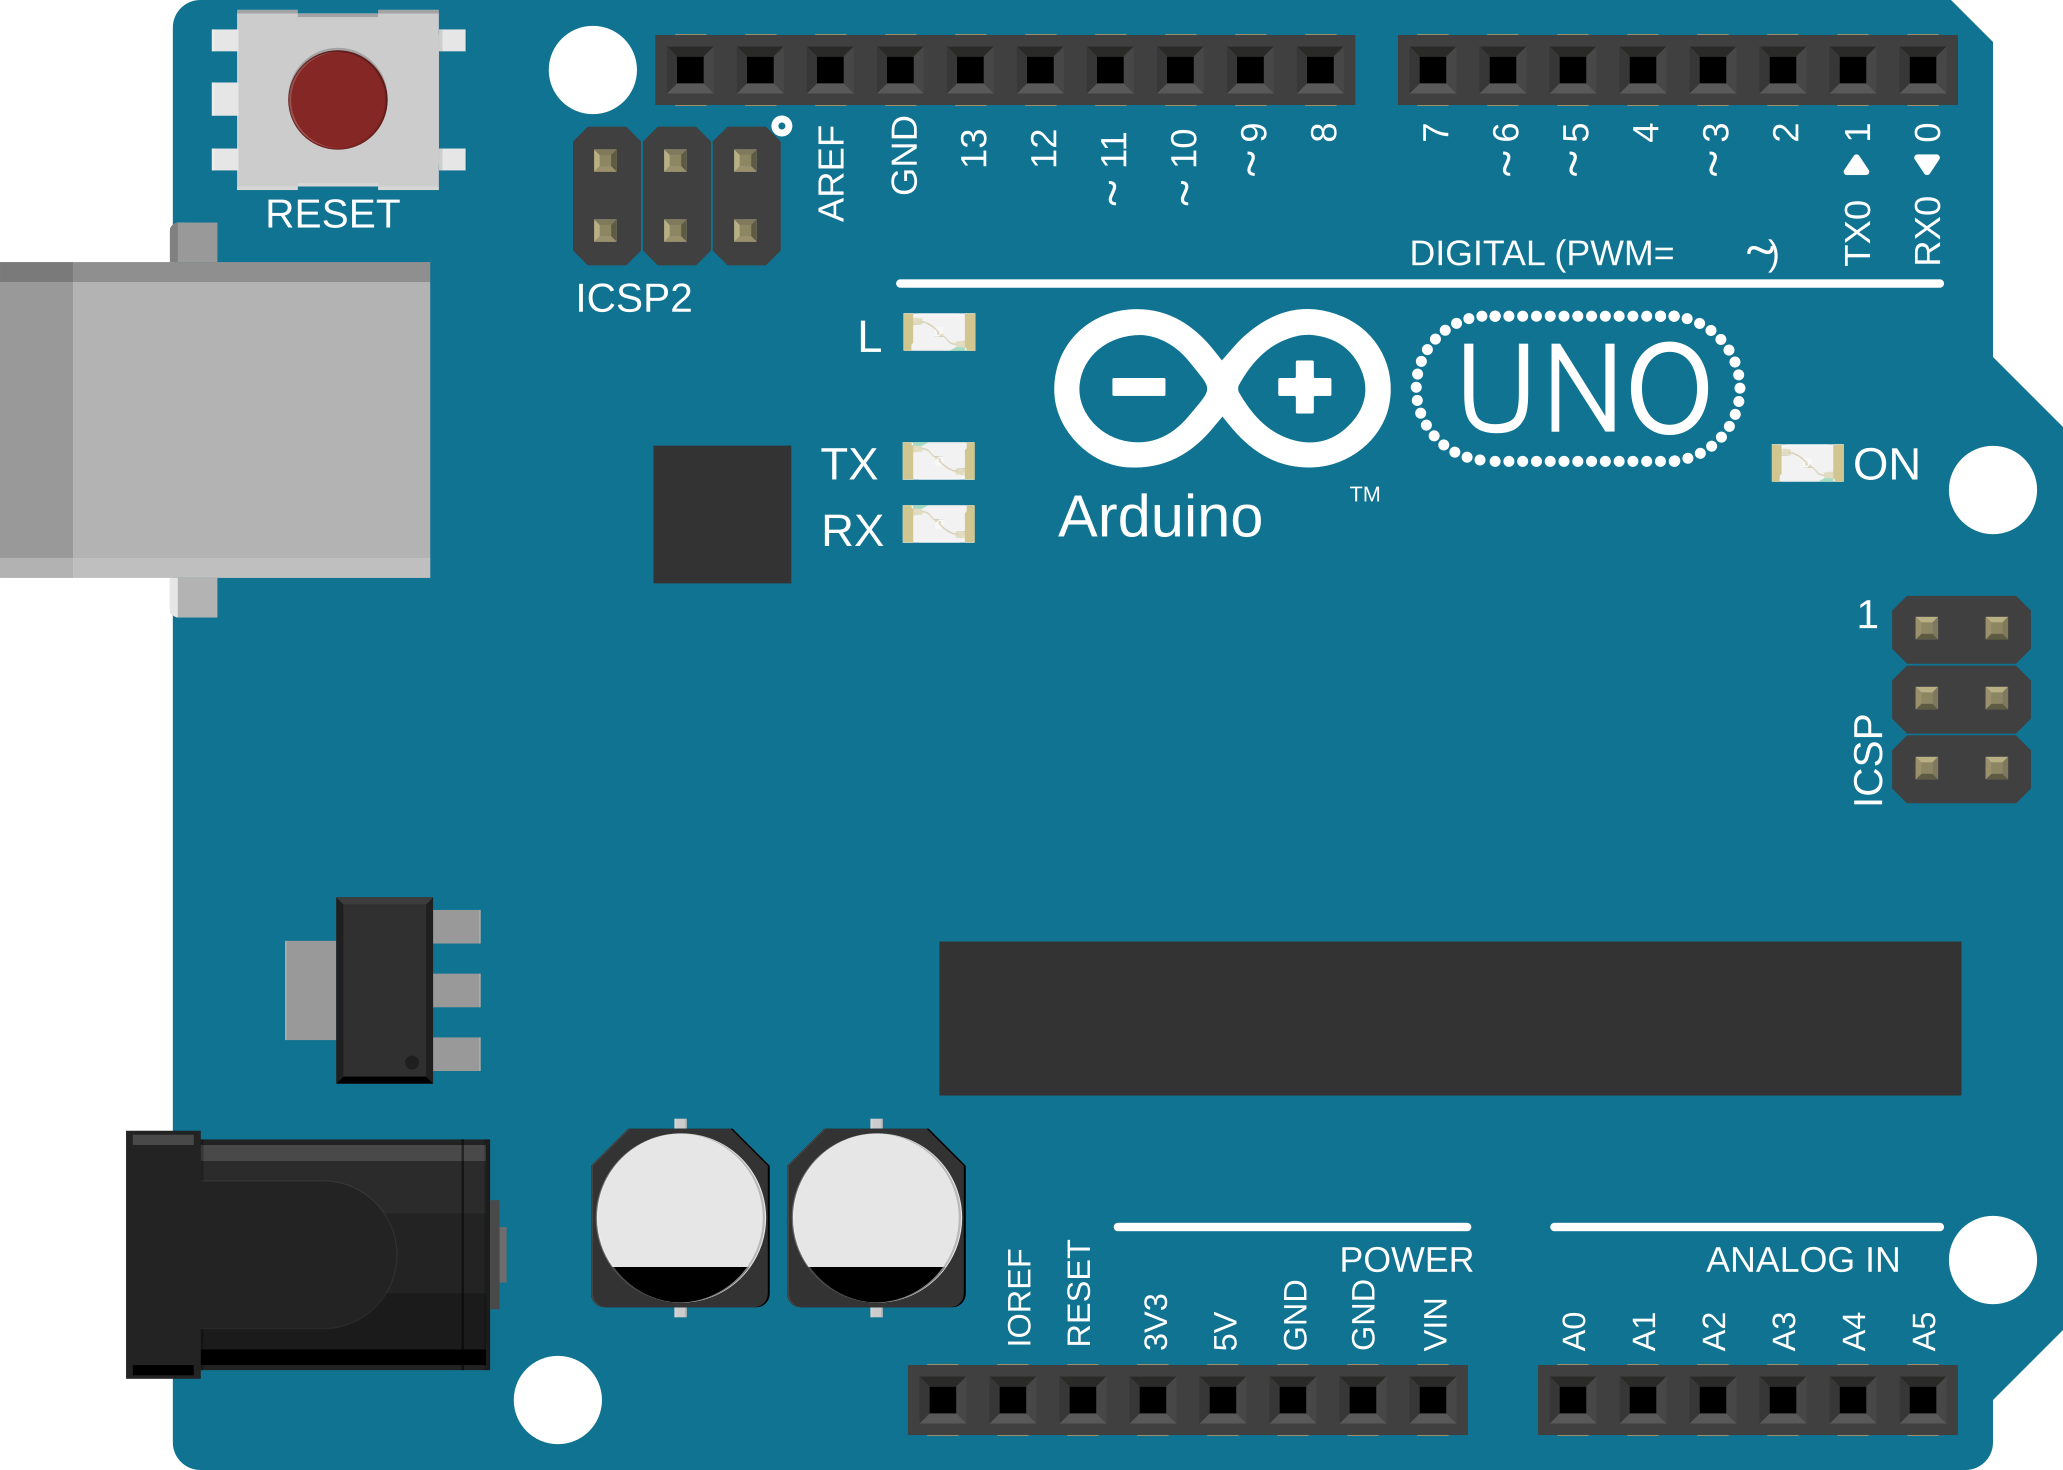
\includegraphics[scale=1.6]{figures/arduino_uno.pdf}
\caption{Arduino UNO mikroupravljačka ploča.\protect\footnotemark}
\label{fig:arduino}
\end{figure}

\footnotetext{Izvorna slika, licencirana pod Creative Commons
    Attribution-ShareALike 3.0 preuzeta je i prilagođena od Fritzing projekta
(\url{https://raw.githubusercontent.com/fritzing/fritzing-parts/master/svg/core/breadboard/arduino_Uno_Rev3_breadboard.svg})}

Na slici \ref{fig:arduino} se vidi Arduino UNO mikroupravljačka ploča. Kao
mikroupravljač koristi se ATmega328 \cite{atmega}. Mikroupravljačka pločica posjeduje 14
digitalnih ulazno/izlaznih pinova, od kojih se 6 mogu koristiti kao pulsno
širinski modulirani izlazi, 6 analognih ulaza, \unit{16}{\mega\hertz} keramički
oscilator, USB sučelje, ulaz za eksterno napajanje i reset tipku. Pločica se
može napajati preko USB sučelja ili preko ulaza za eksterno napajanje.
Komunikacija s računalom odvija se preko USB-serijskog sučelja. Za programski
dio mikroupravljač sadrži \unit{32}{\kilo\byte} flash memorije koje se mogu programirati.

\newpage
\section{Firmata}

Firmata je jednostavan protokol baziran na MIDI-ju i koji je namijenjen za komunikaciju
računala s mikroupravljačem. Cilj mu je omogućiti direktno upravljanje što većim
dijelom mikroupravljača od strane računala.

Za podatkovni format protokola odabrane su MIDI \cite{midi} poruke. Nije u
potpunosti kompatibilan s MIDI standardom, budući da se koristi brža serijska
konekcija i poruke se ne preklapaju u svim slučajevima. No za parsiranje poruka
moguće je koristiti postojeće MIDI parsere.

Protokol se može implementirati kao firmware za bilo koji mikroupravljač ili kao
softver za računalo. Firmata je prvi puta implementirana za mikroupravljače za
Arduino obitelj mikroupravljača. Kao računalni softver, postoji mnogo Firmata 
implementacija za razne jezike, između ostalog i za Python \cite{pyfirmata}
i Haskell \cite{harduino}

\begin{table}[h]
\setlength{\tabcolsep}{18pt}
\centering
    \begin{tabular}{|c|c|}
        \hline
        Naredba               & Numerička vrijednost \\
        \hline
        analog I/O message    & 0xE0 \\
        \hline
        digital I/O message   & 0x90 \\
        \hline
        report analog pin     & 0xC0 \\
        \hline
        report digital port   & 0xD0 \\
        \hline
        start sysex           & 0xF0 \\
        \hline
        set pin mode(I/O)     & 0xF4 \\
        \hline
        set digital pin value & 0xF5 \\
        \hline
        sysex end             & 0xF7 \\
        \hline
        protocol version      & 0xF9 \\
        \hline
        system reset          & 0xFF \\
        \hline
    \end{tabular}
    \caption{Firmata naredbe}
    \label{tbl:firmata}
\end{table}

Na tablici \ref{tbl:firmata} se vide neke od Firmata naredbi i njihove
odgovarajuće numeričke vrijednosti. Da bi se naredio reset mikroupravljača,
jednostavno se preko serijske veze pošalje vrijednost 0xFF te, nakon što
mikroupravljač primi poruku, izvršit će reset rutinu.

\newpage
\section{JSON-RPC}

JSON-RPC je jednostavan protokol za udaljene proceduralne pozive, ne sadržava
stanje i nije definiran kao transportni protokol \cite{jsonRPC}. Koristi JSON
\cite{jsonRFC} kao podatkovni format.

Pozivna poruka sastoji se od:
\begin{itemize}
        \item jsonrpc - verzija protokola
        \item method - ime udaljene metode koja se poziva
        \item params - ulazni parametri za metodu
        \item id - identifikacijska oznaka poruke
\end{itemize}

Ulazni parametri moraju biti strukturiran podatak. Mogu biti u obliku niza ili
JSON objekta, s imenovanim varijablama koje odgovaraju parametrima pozvane
metode.

Odgovor se sastoji od:
\begin{itemize}
    \item jsonrpc - verzija protokola ("2.0")
    \item result - rezultat koji vraća pozvana metoda
    \item error - greška ako ona postoji
    \item id - identifikacijska oznaka poruke
\end{itemize}

Ako dolazi do greške odgovor neće sadržavati rezultat, nego će rezultat će
zamijeniti greška, a svi ostali dijelovi odgovora ostaju isti.
Identifikacijska oznaka u odgovoru mora biti ista kao i u pozivu.

Primjer poziva:
\mint{json}|{"jsonrpc": "2.0", "method": "subtract", "params": [42, 23], "id": 1}|

Tu se vidi poziv koji koristi verziju 2.0 JSON-RPC protokola. Ona poziva metodu
\emph{substract} kojoj predaje parametre u obliku niza (brojčane vrijednosti 42
i 23) te koristi identifikacijsku oznaku s brojem 1.

Primjer odgovora za prethodnu pozivnu poruku:
\mint{json}|{"jsonrpc": "2.0", "result": 19, "id": 1}|

U odgovoru je vidljivo kako server koristi isti protokol kao i klijent, vraća rezultat
pozvane metode te koristi istu identifikacijsku oznaku kao što je dobio u
pozivnoj poruci od klijenta.

